\documentclass{book}
\usepackage[utf8]{inputenc}
\usepackage[spanish]{babel}
\usepackage{graphicx}
\usepackage{graphicx,subfig}
\usepackage{mathptmx}
\usepackage{multicol}
\usepackage{color}
\usepackage{listings}
\usepackage[usenames,dvipsnames,svgnames,table]{xcolor}

\begin{document}
	\thispagestyle{empty}
	\frontmatter
	\begin{minipage}{.3\textwidth}
	\begin{flushleft}
		\begin{center}
			{
\includegraphics[scale=.35]{Assets/images/escudo_unam.png}}
		\end{center}
		\vspace{10pt}
		\begin{center}{
				\rule{.5pt}{.6\textheight}
				\hspace{7pt}
				\rule{2pt}{.6\textheight}
				\hspace{7pt}
				\rule{.5pt}{.6\textheight}
			}
		\end{center}
		\begin{center}{
\includegraphics[scale=1]{Assets/images/escudo_fi.jpg}}\end{center}
	\end{flushleft}
	\end{minipage}
	\begin{minipage}{.7\textwidth}
		\begin{flushright}
				\begin{center}
				\begin{center}
					\LARGE{U}\large{NIVERSIDAD} \LARGE{N}\large{ACIONAL} 
					\LARGE{A}\large{UTÓNOMA} \\[10pt]
					\large{DE} 
					\LARGE{M}\large{ÉXICO} 
				\end{center}
				\rule{\textwidth}{2pt}
				\\
				\hrulefill\\[1cm]
				
				\LARGE{F}\large{ACULTAD DE } \LARGE{I}\large{NGENIERÍA}\\[2cm]
				
				\large{Representación de instrumentos musicales en modelos matemáticos para la generación fidedigna de Música}\\[1.5cm]
				
				\huge{T E S I S }\\[1.5cm]
				
				\large{QUE PARA OBTENER EL TÍTULO DE:}\\[1cm]
				
				\large{INGENIERO EN COMPUTACIÓN}\\[1cm]
				
				\large{PRESENTA}
				
				\large{Joaquín Gustavo Espino de Horta}\\[1cm]
				
				\large{DIRECTOR DE TESIS}
				
				\large{Dr. Rogelio Alcántara Silva}\\[1cm]
				
				\large{Ciudad Universitaria, Cd. Mx., Agosto 2024}
				
			\end{center}
		\end{flushright}
	
	\end{minipage}
	
	
	\pagebreak
	\begin{minipage}{.7\textwidth}
	\begin{flushleft}
		\vspace{10pt}
		\begin{center}
			\Large{INTRODUCCIÓN}
			\hrulefill\\[1.5cm]
		\end{center}
	\end{flushleft}
	\end{minipage}\par
	La propuesta hoy presentada comenzó como una necesidad no resuelta por las herramientas disponibles y demandas hechas por los proyectos de escasos recursos presupuestarios y personal, mejor conocidos como proyectos independientes en los ámbitos de producción en software destinados a la recreación y el ocio como lo son juegos de video y multimedia, a su vez, disponer de una herramienta adicional a los ya indispensables usos del procesador de textos, hojas de cálculo, controlador de diapositivas, entre otros integrados y dependientes exclusivamente del equipo de cómputo. \par
	
	Si bien, este proyecto no es pionero en su finalidad, en lo que a producción de origen totalmente computacional es referido, la composición de obras auditivas en formatos digitales sigue siendo parcialmente dependiente de la captura y edición de la información proveniente de los instrumentos musicales físicos capturados por periféricos especializados, donde en estos se requiere un compromiso absoluto en la disciplina artística, así como la ingeniería propia involucrada en el muestreo y alteración en las señales de audio.\par
	
	Existen algunas herramientas de porte comercial dedicadas a la generación del audio sin la demanda de un instrumento o captura de este, aun así, estas no ha sido diseñadas en dotar a su producto de una calidad definitiva, pues ha sido concebida como una referencia o prueba de concepto, pues el método de producción basado en la adición estratégica con muestras pre-grabadas de notas musicales, tienen una clara limitante en cuanto a tiempo, diversidad en variaciones de interpretación entre muchos aspectos no deseados en vista a un producto final, pues a nivel de consumidor, no sería de su agrado la escucha de sonidos tan parecidos y sin sus variaciones.\par
	
	Esta problemática no refiere a una urgencia en el mercado, aunque si aspira a la dar un nuevo abanico de opciones en cuanto la producción musical, una que permita cubrir la sincronización con el tiempo así como la correcta interpretación de sonidos hechos en instrumentos musicales, en otras palabras, dar a los compositores sean aspirantes o expertos la posibilidad de aumentar e inaugurar una mayor y más eficiente producción, brindando las bondades que nos ha traído la programación informática, referentes al propio soporte, el trabajo re-utilizable incluso en cuanto a un nuevo paradigma de almacenamiento y respuesta computacional adecuada a los temas sonoros.\par
	
	Véase un anuncio publicitario compuesto con los \emph{jingles} establecidos de la corporación, el repertorio cultural en potencia al disponer a cada usuario las herramientas para componer la futura obra maestra en una industria saturada por el monopolio de tendencias actuales, surgidas en culturas y lugares distintos, todo disponible desde la misma plataforma y capacidades de la máquina capaz de ejecutar un editor de textos comercial.\par
	
	Después de todo, ya existen los conjuntos de herramientas totalmente independientes para la elaboración de sus respectivos productos, hablando también de aquellos más complejos como obras audiovisuales, construcción de modelos en tres dimensiones o combinando todos estos para la elaboración de aplicaciones gráficas orientadas al entretenimiento, mejor conocidos como \emph{videojuegos}\par
	
	\pagebreak
	\begin{minipage}{.7\textwidth}
		\begin{flushleft}
			\vspace{10pt}
			\begin{center}
				\Large{VISIÓN}
				\hrulefill\\[1.5cm]
			\end{center}
		\end{flushleft}
	\end{minipage}\par
	La siguiente imagen muestra una representación simplificada sobre la propuesta de solución al completo, donde se tiene planeadas todas sus funcionalidades y operaciones al menos de cara a un lanzamiento hacia el público interesado, más no uno comercial.\par
	
	Están contempladas 5 grandes aspectos para el desarrollo de una aplicación integral, aunque se aclara desde este punto, solo se centrará en un módulo, el más significativo en cuanto una nueva propuesta se refiere. Siendo el módulo de \emph{Tuner} (afinador).
	\begin{figure}[h]
		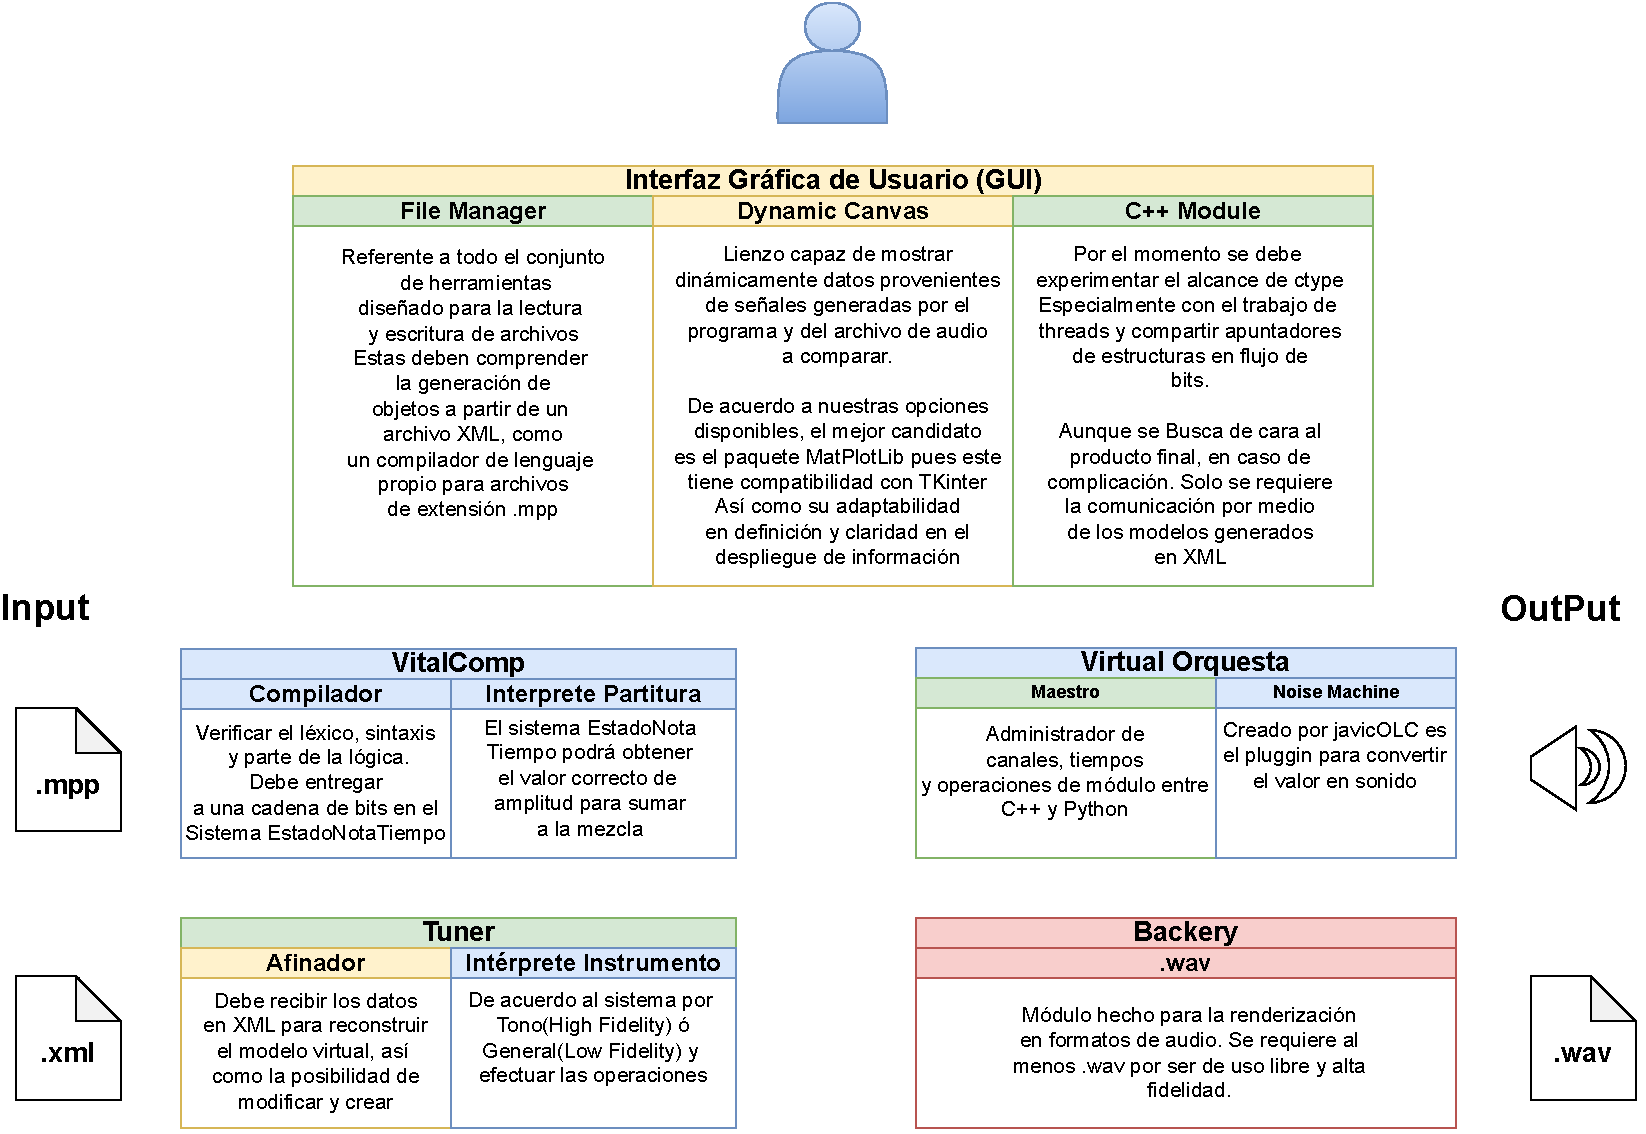
\includegraphics[width=1.25\linewidth]{Assets/images/musiC++_Diagram}
		\caption{ Diagrama General del Proyecto Completo}
	\end{figure} 
	
	\pagebreak
	\begin{minipage}{.7\textwidth}
		\begin{flushleft}
			\vspace{10pt}
			\begin{center}
				\Large{MÓDULOS}
				\hrulefill\\[1.5cm]
			\end{center}
		\end{flushleft}
	\end{minipage}\par
	Profundizando en los módulos mostrados anteriormente:\par
	{\Large Interfaz Gráfica de Usuario (GUI)}\par
	El enfoque comercial del proyecto, exige que este contenga por lo menos una visualización cercana a los estándares en herramientas de software, si bien, el público general cambia su tendencia en cuanto conocimientos informáticos básicos, sería un error cerrarnos de cara a una presentación como la manipulación para una terminal de consola. Se ha experimentado construir una GUI con el lenguaje \emph{C++}, sin embargo no pudo encontrarse una biblioteca adecuada, mucho menos un resultado satisfactorio para delegar todo el proyecto a un único lenguaje de programación, por lo tanto, se trabajará con Python en el \emph{FrontEnd}, es decir, todo contacto con el usuario final.\par
	{\large File Manager}\par
	Ya que nuestro propósito es la generación de archivos cuya información pueda interpretarse por un estándar orientado a audio, así como la preservación del trabajo en un lenguaje de programación, es imperativo usar varios sistemas de lectura y escritura de archivos en ambos lenguajes a utilizar, siendo \emph{Python} y \emph{C++}, estos contienen una biblioteca en sus paquetes fundamentales, siendo la función \emph{open} y \emph{fstream} respectivamente. Por otra parte, se necesitará de una biblioteca especializada en convertir la información de un texto etiquetado como lo es el formato XML. No solo es un estándar que permite escalar las funciones del proyecto a futuro con otros productos de software, sino que al ser un formato simple y en cierto punto, indicativo para ser editado manualmente.\par
	{\large Dynamic Canvas}\par
	Si bien, esta parte podría únicamente ser útil en lo que respecta la construcción del módulo afinador. Puede utilizarse en tiempo real la representación gráfica de la información generada, desde los armónicos que participan en la mezcla del sonido, una visión más amigable de cara al usuario de los eventos programados, entre otras cosas. Ya que esto está ligado a la GUI así como el afinador, su desarrollo sería exclusivamente en Python, optando por la opción que ofrece el paquete de MatPlotLib por su compatibilidad con TKinter\par
	{\large C/C++ Module}\par
	Debido a las características por implementar, es conveniente dejar a Python como aquel que tenga el ejecutable inicial, así como ser el eje de las herramientas que conlleve el proyecto. Este ofrece una opción denominada como \emph{ctype} el cual permite convocar código en \emph{C/C++} colocando y devolviendo datos primitivos, aún no se ha experimentado del todo, pues se requiere de la certeza y técnicas en cuanto el envío de apuntadores para arreglos de datos, estructuras específicas así como su correcto funcionamiento con múltiples hilos de ejecución.
	
	\pagebreak{\Large VitalComp}\par
	Este módulo comprende el lenguaje de programación propuesto para la codificación de melodías en cuanto Tonos y Tiempos se refiere, así como su manejo en melodías. El nombre es en conmemoración a un profesional en la música, conocido personal, \emph{Vitalis Elrich} a quien se le había consultado la idea inicial y gracias al estudio de necesidades y herramientas actuales en el mercado, se sugirió la propuesta sobre un lenguaje de programación.\par
	{\large Compilador}\par
	El compilador estará compuesto por 2 fases (independientes al análisis léxico, semántico y lógico), pues se plantean 2 paradigmas distintos en un mismo formato, pues por un lado tendríamos las necesidades logísticas en cuanto a la sincronización, designación de tiempos, incluso la posibilidad de implementar una aritmética y lógica primordiales con el fin de hacer compatible con otros códigos.
	Para su construcción, se emplearán los recursos de \emph{Flex} y \emph{Bison} para las primeras etapas, donde se obtendrá una cadena atómica verificada en la que se interpretarán parcialmente los comandos y símbolos para la adecuación del ambiente al momento de recibir la segunda fase, esta consistirá en reconocer elementos melódicos como el nombre de las notas(pueden ser católicas o protestantes), comandos referentes a acordes específicos, así como la duración, varianza en semitonos entre otras características que pueda contener una partitura y ser representada en comandas. Para este último conviene manejarse en un detector de símbolos para la reducción atómica y el complemento en una cadena de Bytes, por medio de un estado universal que tenga tiempos por defecto así como los propios modos... Así estamos solucionando el uso dinámico pues al ejecutarse condicionalmente, la computadora podrá re-compilar las partes móviles\par
	{\large Intérprete}\par
	Ajustando el proyecto original del usuario \emph{Javidx9/OneLoneCoder}, se parte de modificar la estructura \emph{sequencer}, cuya función principal es la generación automática de información en tiempos y notas para que sean añadidas en el mecanismo principal. Si bien, su versión está limitada a una sola característica, pues fue diseñada como un efecto cíclico de batería. Rescatando el concepto abstracto del secuenciador, es posible modificar a un sistema de interpretación por cadenas de Bytes, inspirado en el \emph{pipeline de renderizado} usado en procesos gráficos de \emph{OpenGL}. Esta consiste en la toma de 3 Bytes con información de tipo Estado, Timbre y Duración, por cada Tempo en secuencia de melodía, es decir, que clase de sonidos, su tiempo en reproducción y el estado técnico para poder formar acordes, silencios o incluso solicitar una interpretación especial(fuera de mayores ó bemoles) en relación con otras notas. Cabe abordar una sugerencia en cuanto la optimización del caso estático, pues si la máquina no contiene ninguna variación, porque de ser el propósito: generar un archivo en memoria de almacenamiento, entonces, no debería compartir el mismo mecanismo en tiempo real, ahorrando recursos de presentación y otorgando una mayor eficiencia de uso.\par
	
	\pagebreak{\Large Virtual Orquesta}\par
	Este es un módulo enfocado al procesamiento central de la información, pues estará diseñado para invocar la interpretación de las instrucciones y ajustes dados por el usuario, administración de los múltiples hilos dedicados, pausa, reinicio, incluso a la captura en tiempo real de notas generadas por el usuario mediante una entrada estándar así como la posibilidad de escalar a un instrumento especializado.\par
	{\large MasterChord}\par
	Siendo esta parte administrativa, deberá cumplir con una facilidad de funciones que puedan ser citadas como servicios desde la GUI así como la respuesta de información siendo instrumentos, posición de notas, tiempo real o cualquier información correspondiente a una visualización con propósitos artísticos o técnicos. Si bien las funciones gráficas son prescindibles, se deja abierta la posibilidad de escalar al producto final.\par
	{\large NoiseMachine}\par
	Esta es una cabecera hecha por \emph{Javidx9/OneLoneCoder} que nos permite la comunicación con el hardware hecho para la reproducción de audio mediante la solicitud del tiempo en valor de la amplitud otorgado por una función asignada. Esta pieza limita el proyecto a plataformas con sistema operativo Windows 7 en adelante, con compatibilidad para arquitectura de x32 bits.\par
	{\large Backery}\par
	Recordando los propósitos iniciales, es evidente la necesidad de respaldar los archivos en memoria de almacenamiento, por lo tanto necesitamos de alguna forma, guardar la información en un estándar para la reproducción de audio.\par
	
	\pagebreak{\Large Tuner}\par
	{\large Generador de Señales}\par
	{\large Virtual Instrument}\par
	
	\pagebreak Para la realización de estos se ha tomado como base un proyecto para emulación de instrumentos del talentoso ingeniero inglés conocido en sus redes sociales electrónicas como \emph{Javidx9}. Su proyecto \emph{olcNoiseMaker} sienta los principios para estos requisitos:\vspace{2mm}
	
	\textbf{Maestro del Audio}
	{\tiny \lstinputlisting[language=c, firstline=381, lastline=403]{Assets/code/main4.cpp}}
	\textbf{Plantilla de Instrumento}
	{\tiny\lstinputlisting[language=c, firstline=183, lastline=209]{Assets/code/main4.cpp}\pagebreak}
	\textbf{Acceso a Hardware}
	{\tiny\lstinputlisting[language=c, firstline=183, lastline=252]{Assets/code/olcNoiseMaker.h}\pagebreak}
	\pagebreak\section{Resultados Esperados}
	El producto en su finalidad debe ser capaz de:
	\begin{itemize}
		\item Bajo en consumo de recursos computacionales
		\item Utilizable en muchos entornos de programación
		\item Facilidad en su comprensión para el usuario
		\item Simulación de instrumentos musicales diversos
		\item Diseño escalable al número de funciones y modos
		\item Grabar los formatos más utilizados en la actualidad
	\end{itemize}
	Respecto a la funcionalidad, esta deberá estar accionada desde una entrada estándar en cadena de texto. Dando como una salida la reproducción del sonido esperado, como su posibilidad de almacenarse en los formatos objetivo.\vspace{2mm}
	
	De esta manera, se espera un uso por parte de usuarios desde aplicaciones sofisticadas con una interfaz gráfica de usuario agradable a la vista, como las opciones comerciales presentadas hasta la implementación en lenguaje de alto nivel. Se tiene como panorama el paradigma de interpretación y lectura secuencial gracias a sus propiedades fundamentales arraigadas en las características de computadoras comerciales accionadas por sistemas Linux ó Windows, así como su vista hacia Android.\vspace{2mm}
	
\end{document}

